\documentclass[tikz,convert={outfile=schematic.svg}]{standalone}
\usetikzlibrary{backgrounds}
%\usetikzlibrary{...}% tikz package already loaded by 'tikz' option
\begin{document}
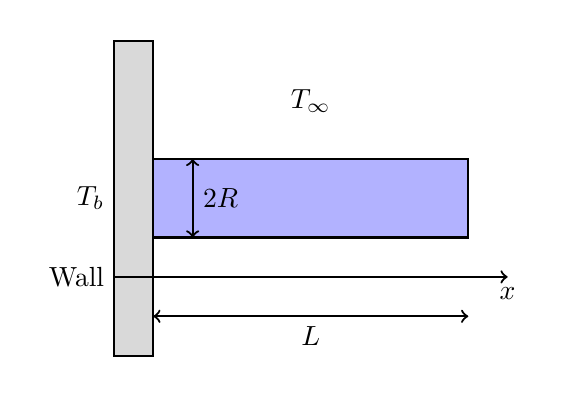
\begin{tikzpicture}[background rectangle/.style={fill=white}, show background rectangle]
  % Define parameters
  \def\L{4}  % Length of the fin
  \def\a{0.5} % Half-thickness of the fin

  % Draw the wall
  \fill[gray!30] (-0.5, -2) rectangle (0, 2);

  % Draw the fin
  \fill[blue!30] (0, -\a) rectangle (\L, \a);

  % Draw x and y axes
  \draw[->, thick] (-0.5, -1) -- (\L + 0.5, -1) node[anchor=north] {$x$};

  % Add labels for dimensions
  \draw[<->, thick] (0, -1.5) -- (\L, -1.5) node[midway, below] {$L$};
  \draw[<->, thick] (0.5, -\a) -- (0.5, \a) node[midway, right] {$2R$};

  % Add temperature annotations
  \node[anchor=east] at (-0.5, 0) {$T_b$};
  \node[anchor=north] at (\L/2, 1.5) {$T_\infty$};

  % Add wall label
  \node[anchor=east] at (-0.5, -1) {Wall};

  % Draw outlines
  \draw[thick] (-0.5, -2) -- (-0.5, 2) -- (0, 2) -- (0, -2) -- cycle;
  \draw[thick] (0, -\a) -- (\L, -\a) -- (\L, \a) -- (0, \a) -- cycle;

\end{tikzpicture}
\end{document}